\documentclass[11pt]{exam}

\usepackage{amsmath}
\usepackage{graphicx}
\usepackage{geometry}
\usepackage{etoolbox}
\BeforeBeginEnvironment{choices}{\par\nopagebreak\minipage{\linewidth}}
\AfterEndEnvironment{choices}{\endminipage}
\geometry{
a4paper,
total={185mm,257mm},
left=10mm,
top=25mm,
bottom=10mm
}

\begin{document}
\setlength{\voffset}{-0.5in}
\setlength{\headsep}{5pt}

\fbox{\fbox{\parbox{8cm}{\centering
\vspace{2mm}
Testat - Versuch D - Zeitabhaengiger Strom - 3
\vspace{2mm}
}}}
\hspace{2mm}
\makebox[0.25\textwidth]{Name:\enspace\hrulefill} \hspace{5mm}
\makebox[0.2\textwidth]{Datum:\enspace\hrulefill}
\vspace{4mm}

\begin{questions}

\question Welche der folgenden Aussagen ist falsch?

\begin{choices}
	\choice Die Kapazität eines Kondensators trägt die Einheit Farad.
	\choice Je größer die Kapazität des Kondensators in einem RC-Glied ist, desto größer ist die Zeitkonstante.
	\choice Wenn die Spannung an einem Kondensator erhöht wird, bleibt die Kapazität konstant.
	\choice Eine Wechselspannung wird durch Angabe der Frequenz, Amplitude und Phase vollständig beschrieben. (correct)
	\choice Je größer der Widerstand in einem RC-Glied ist, desto größer ist die Zeitkonstante.
\end{choices}

\vspace{3mm}\question Ein zeitlich konstanter Strom \(\mathrm{I}\) fließt in einen Kondensator mit einer Kapazität von \(\mathrm{C=1\,mF}\) und lädt diesen auf. Nach der Zeit \(\mathrm{t=10\,s}\) beträgt die Spannung am Kondensator \(\mathrm{U=100\,V}\). Wie groß war der Strom \(\mathrm{I}\)?\(\mathrm{Q=C \cdot U}\) und \(\mathrm{Ampere=Coulomb/Sekunde}\).

\begin{choices}
	\choice \(\mathrm{1\,mA}\)
	\choice \(\mathrm{1\,A}\)
	\choice \(\mathrm{10\,mA}\) (correct)
	\choice \(\mathrm{100\,mA}\)
	\choice \(\mathrm{10\,A}\)
\end{choices}

\vspace{3mm}\question Welche Frequenz hat das auf dem Oszilloskop gezeigte Signal? Der Skalierungsfaktor für die X-Achse beträgt \(\mathrm{0,2\,ms/DIV}\), der Skalierungsfaktor für die Y-Achse beträgt \(\mathrm{5\,V/DIV}\). 

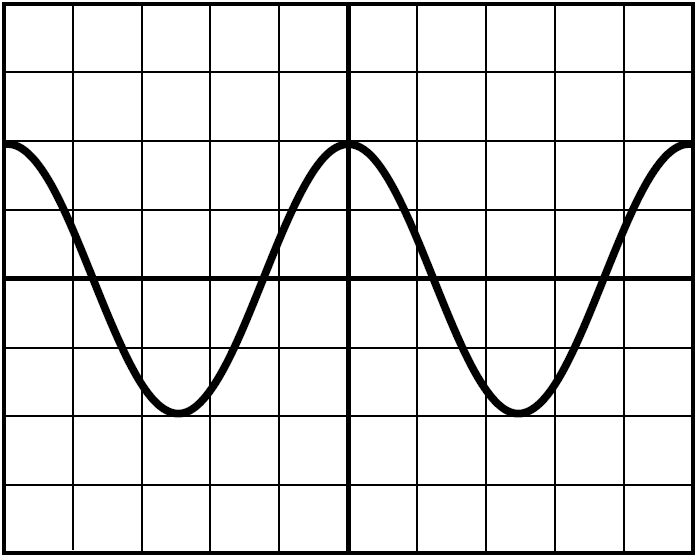
\includegraphics[width=0.5\textwidth]{../../../questions/D/images/Oszi2.png}

\begin{choices}
	\choice \(\mathrm{2\,ms}\)
	\choice \(\mathrm{1\,kHz}\) (correct)
	\choice \(\mathrm{500\,Hz}\)
	\choice \(\mathrm{2\,kHz}\)
	\choice \(\mathrm{1\,ms}\)
\end{choices}

\vspace{3mm}\question In welchen Einheiten werden üblicherweise die Membranzeitkonstante, die Membranlängskonstante und die Reizleitgeschwindigkeit angegeben?

\begin{choices}
	\choice Membranzeitkonstante in \(\mathrm{s}\), Membranlängskonstante in \(\mathrm{mm}\), Reizleitgeschwindigkeit in \(\mathrm{V/s}\)
	\choice Membranzeitkonstante in \(\mathrm{s}\), Membranlängskonstante in \(\mathrm{mm}\), Reizleitgeschwindigkeit in \(\mathrm{m/s}\) (correct)
	\choice Membranzeitkonstante in \(\mathrm{s^{-1}}\), Membranlängskonstante in \(\mathrm{mm^{-1}}\), Reizleitgeschwindigkeit in \(\mathrm{V/s}\)
	\choice Membranzeitkonstante und Membranlängskonstante haben keine Einheit, Reizleitgeschwindigkeit in \(\mathrm{m/s}\)
	\choice Membranzeitkonstante in \(\mathrm{s^{-1}}\), Membranlängskonstante in \(\mathrm{mm^{-1}}\), Reizleitgeschwindigkeit in \(\mathrm{m/s}\)
\end{choices}

\vspace{3mm}\question Welcher der folgenden Kurvenverläufe gibt die Ladekurve eines Kondensators, der mit einem konstanten Strom geladen wird, qualitativ richtig wieder? 

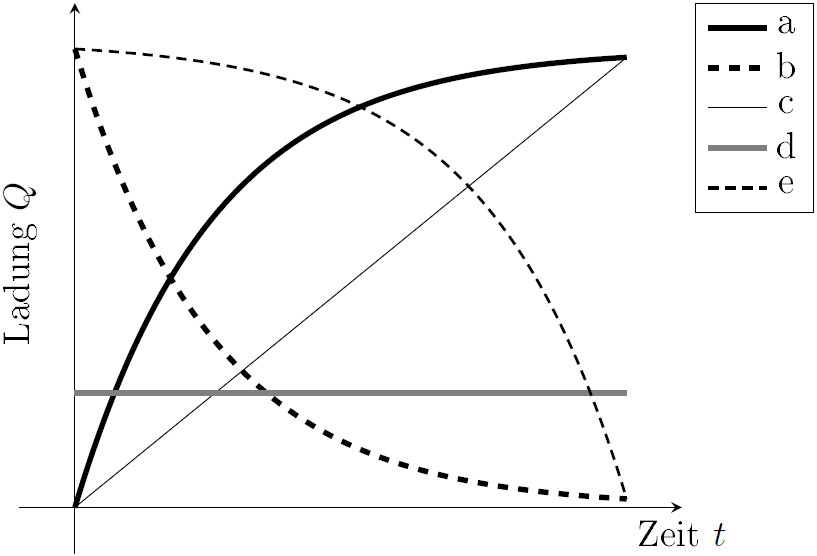
\includegraphics[width=0.5\textwidth]{../../../questions/D/images/Kondensator-Q-t.png}

\begin{choices}
	\choice a
	\choice e
	\choice b
	\choice c (correct)
	\choice d
\end{choices}

\vspace{3mm}\end{questions}

\end{document}
